%!TEX root = ../thesis.tex

本章では, 従来研究を基にしたオフラインでデータを収集し訓練する手法を提案する.

\section{手法}
本研究で提案する手法を述べる. 従来手法に対して, 提案手法は一度にデータを収集して, オフラインで訓練することが異なる. 
\par \figref{Fig:collect-data2}にデータの収集方法を示す. 赤色の線である目標経路から平行に離れた座標にロボットを配置する. そして, その座標ごとに64×48のカメラ画像(RGB画像)とルールベース制御器によるナビゲーションの出力である角速度を\figref{Fig:collect-data2}のように収集する. ロボットの進行方向に対する並進速度は0m/sであるが, データセットにはナビゲーションの出力である角速度がロボットに与えられる. \par このように, ロボットを走行させることなく, 目標経路上及び周辺に配置することで, 一度に大量のデータを収集することができる. その後, 収集したデータを用いてオフラインで学習を行う. また, 従来研究ではオンラインで学習を行うため, 計算のリソースなどの観点からバッチサイズを8にして, 全てのデータを利用してなかった(以下「従来の学習方法」と称する). しかし, 提案手法ではオフラインで学習を行うため, バッチ学習を用いた訓練も試みる. 

% \vspace{10mm}
\newpage
  \begin{figure}[h]
  \centering
  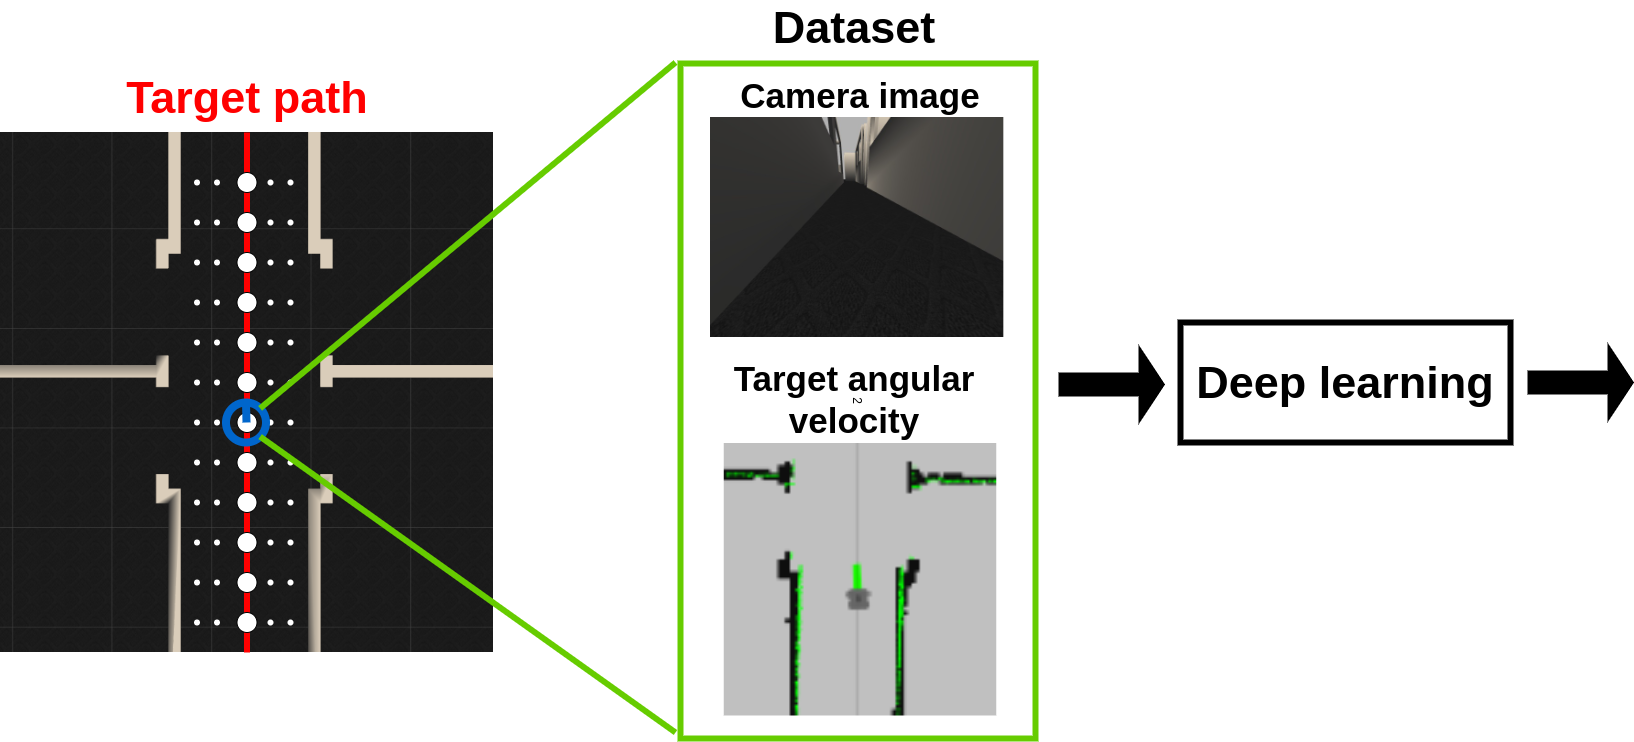
\includegraphics[keepaspectratio, scale=0.25]{images/collect-data2.png}
  \caption{Method of collecting data around the target route}
  \label{Fig:collect-data2}
  \end{figure}

